\documentclass[11pt, norsk]{article}
%\usepackage[latin1]{inputenc}
\usepackage[T1]{fontenc}
\usepackage[utf8]{inputenc}
\usepackage[norsk]{babel}   % S P R A A K


% \usepackage{graphicx}    % postscript graphics
\usepackage{amssymb, amsmath, amsthm, amssymb} % symboler, osv
\usepackage{mathrsfs}
\usepackage{url}
\usepackage{thmtools}
\usepackage{enumerate}  % lister $  
\usepackage{float}
\usepackage{tikz}
\usetikzlibrary{calc}
\usepackage{tikz-3dplot}
\usepackage{subcaption}
\usepackage[all]{xy}   % for comm.diagram
\usepackage{wrapfig} % for float right
\usepackage{hyperref}
\usepackage{mystyle} % stilfilen      


\begin{document}
\title{Oppgaver MAT2500}
\author{Fredrik Meyer}
\maketitle 
\begin{oppg}
Beskriv et polyeder med $5$ hjørner og $6$ sider der alle sidene er trekanter. Beskriv to polyedre med $6$ hjørner og $8$ sider der alle sidene er trekanter.
\end{oppg}
\begin{losn}
Vi vet fra Eulers formel at det alltid gjelder at
\[
v-e+f = 2
\]
for konvekse polyedre. Her er $v$ antall hjørner, $e$ er antall kanter, og $f$ er antall flater. Dermed finner vi at den første figuren må ha $9$ kanter. Dette gir oss en ide om hva det kan være, og etter litt tenking skjønner vi at et svar er den rette dobbelpyramiden på en trekant. Se Figur 1.

På samme måte ser vi at et polyeder med $6$ hjørner og $8$ sider må ha $12$ kanter. Ett slikt polyeder er oktaeder, som vi har tegnet i Figur 2. 

Vi har derimot to muligheter. Den andre muligheten er ikke regulær, da det her finnes to hjørner som møter $5$ kanter (i oktaederet møter alle hjørner $4$ kanter). Se Figur 3.

\begin{figure}
\begin{center}

\tdplotsetmaincoords{81}{127}
  \begin{tikzpicture}[scale=5,tdplot_main_coords]

    \draw[thick,->] (0,0,0) -- (1,0,0) node[anchor=north east]{$x$};
    \draw[thick,->] (0,0,0) -- (0,1,0) node[anchor=north west]{$y$};
    \draw[thick,->] (0,0,0) -- (0,0,1) node[anchor=south]{$z$};

   \coordinate (A) at (-0.5,-{sqrt(3)/6},0);
   \coordinate (B) at (0.5,-{sqrt(3)/6},0);
   \coordinate (C) at (0,{sqrt(3)/3},0);
   \coordinate (E) at (0,0,{sqrt(2/3)});
   \coordinate (F) at (0,0,-{sqrt(2/3)});

\draw[dashed, red] (A) -- (B);
\draw[thick, red] (B) -- (E);
\draw[dashed, red] (E) -- (A);
\draw[thick, red]  (B) -- (F);
\draw[dashed, red]  (A) -- (F);
\draw[thick, red] (C) -- (F);
\draw[thick, red] (C)  -- (E);
\draw[dashed, red] (C)  -- (A);
\draw[thick, red] (C)  -- (B);

  \end{tikzpicture}
\end{center}
\caption{Den rette bipyramiden på en regulær trekant.}
\end{figure}

\begin{figure}
\begin{center}

\tdplotsetmaincoords{81}{127}
  \begin{tikzpicture}[scale=3,tdplot_main_coords]

%    \draw[thick,->] (0,0,0) -- (1,0,0) node[anchor=north east]{$x$};
%    \draw[thick,->] (0,0,0) -- (0,1,0) node[anchor=north west]{$y$};
%    \draw[thick,->] (0,0,0) -- (0,0,1) node[anchor=south]{$z$}; 

   \coordinate (A) at (1,1,0);
   \coordinate (B) at (-1,1,0);
   \coordinate (C) at (-1,-1,0);
   \coordinate (D) at (1,-1,0);
   \coordinate (E) at (0,0,{sqrt(2)});
   \coordinate (F) at (0,0,-{sqrt(2)});

\draw[red] (D) -- (A) -- (B);
\draw[dashed, red] (B) -- (C) -- (D);
\draw[red] (E) -- (A);
\draw[red] (E) -- (B);
\draw[dotted,red] (E) -- (C);
\draw[red] (E) -- (D);
\draw[red] (F) -- (A);
\draw[red] (F) -- (B);
\draw[dotted,red] (F) -- (C);
\draw[red] (F) -- (D);

  \end{tikzpicture}
\end{center}
\caption{Et oktaeder.}
\end{figure}

\begin{figure}
\begin{center}

\tdplotsetmaincoords{100}{200}
  \begin{tikzpicture}[scale=3,tdplot_main_coords]

%    \draw[thick,->] (0,0,0) -- (1,0,0) node[anchor=north east]{$x$};
%    \draw[thick,->] (0,0,0) -- (0,1,0) node[anchor=north west]{$y$};
%    \draw[thick,->] (0,0,0) -- (0,0,1) node[anchor=south]{$z$}; 

   \coordinate (A) at ({(1/4)*sqrt(10+2*sqrt(5))},{0.25*(sqrt(5)-1)},0);
   \coordinate (B) at (0,1.1,-0.1);
   \coordinate (C) at (-{(1/4)*sqrt(10+2*sqrt(5))},{0.25*(sqrt(5)-1)},0);
   \coordinate (E) at (-{(1/4)*sqrt(10+2*sqrt(5))},{-0.25*(sqrt(5)-1)},0);
   \coordinate (F) at ({(1/4)*sqrt(10+2*sqrt(5))},{-0.25*(sqrt(5)-1)},0);
   \coordinate (D) at (0,0,1);

\draw[thick, red] (A) -- (B) -- (C) -- (E) -- (F) -- cycle;
\fill[green, opacity=0.2] (A) -- (B) -- (C) -- (E) -- (F) -- cycle;
\fill[blue, opacity=0.2] (D) -- (E) -- (F) -- cycle;
\fill[red, opacity=0.2] (D) -- (E) -- (C) -- cycle;
\fill[orange, opacity=0.2] (D) -- (C) -- (B) -- cycle;
\fill[yellow, opacity=0.2] (D) -- (B) -- (A) -- cycle;
\fill[pink, opacity=0.2] (D) -- (A) -- (F) -- cycle;
\fill[black, opacity=0.2] (B) -- (C) -- (E) -- cycle;
\fill[black, opacity=0.2] (B) -- (E) -- (F) -- cycle;
\fill[black, opacity=0.2] (B) -- (F) -- (A) -- cycle;
\draw (D) node[above] {T} -- (A);
\draw (D) -- (B);
\draw (D) -- (C);
\draw (D) -- (E);
\draw (D) -- (F);
\draw[dashed] (B) -- (E);
\draw[dashed] (B) -- (F);

  \end{tikzpicture}
\end{center}
\caption{Pyramide på et ``skjevt'' pentagon.}
\end{figure}
\end{losn}

\begin{oppg}
Tegn Schlegel-diagrammer for de $5$ platonske legemene.
\end{oppg}

\begin{losn}
Å gjøre dette nøyaktig er en så tidkrevende jobb at selv datamaskiner puster tungt. Det som er interessant i Schlegel-diagrammet er den kombinatoriske strukturen til polytopene, og dette kan vi lett tegne inn. 

Se Figurene 4,5,6. Teknikken for de to siste er slik: legg merke til at i alle hjørnene møtes et fast antall mangekanter. Dette bestemmer hele strukturen, og du kan arbeide deg innover. (prøv selv!)

\begin{figure}
\centering
\begin{subfigure}[b]{0.3\textwidth}
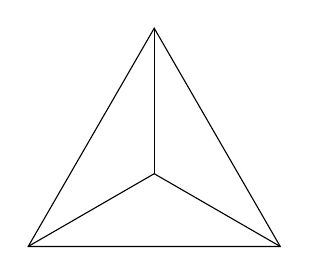
\begin{tikzpicture}[scale=0.8]
\coordinate (A) at (2,0);
\coordinate (B) at (-2,0);
\coordinate (C) at (0,{2*sqrt(3)});
\coordinate (D) at (0,{2*sqrt(3)/3});

\draw (A) -- (B) -- (C) -- cycle;
\draw (A) -- (D);
\draw (B) -- (D);
\draw (C) -- (D);

\end{tikzpicture}
\caption{Tetraeder.}
\end{subfigure}
\begin{subfigure}[b]{0.3\textwidth}
  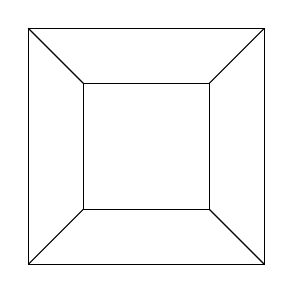
\begin{tikzpicture}
 \coordinate (A) at (1.5,1.5);
 \coordinate (B) at (-1.5,1.5);
 \coordinate (C) at (-1.5,-1.5);
 \coordinate (D) at (1.5,-1.5);
 \coordinate (E) at (0.8,0.8);
 \coordinate (F) at (-0.8,0.8);
 \coordinate (G) at (-0.8,-0.8);
 \coordinate (H) at (0.8,-0.8);

\draw (A) -- (B) -- (C) -- (D) -- cycle;
\draw (E) -- (F) -- (G) -- (H) -- cycle;
\draw (A) -- (E);
\draw (B) -- (F);
\draw (C) -- (G);
\draw (D) -- (H);
  \end{tikzpicture}
\caption{Kube.}
\end{subfigure}
\begin{subfigure}[b]{0.3\textwidth}
  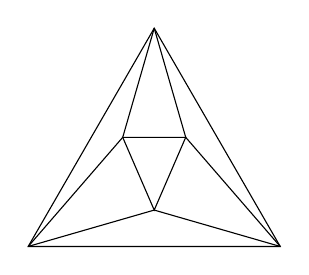
\begin{tikzpicture}[scale=0.8]
\coordinate (A) at (2,0);
\coordinate (B) at (-2,0);
\coordinate (C) at (0,{2*sqrt(3)});
\coordinate (D) at (0,{2*sqrt(3)/6});
\coordinate (E) at (-0.5,{4*sqrt(3)/4});
\coordinate (F) at (0.5,{4*sqrt(3)/4});

\draw (A) -- (B) -- (C) -- cycle;
\draw (A) -- (D);
\draw (A) -- (F);
\draw (B) -- (D);
\draw (B) -- (E);
\draw (C) -- (E);
\draw (C) -- (F);
\draw (D) -- (E) -- (F) -- cycle;

  \end{tikzpicture}
\caption{Oktaeder.}
\end{subfigure}
\caption{Schlegel-diagrammer for de tre første platonske legemene.}
\end{figure}

\begin{figure}
\centering
  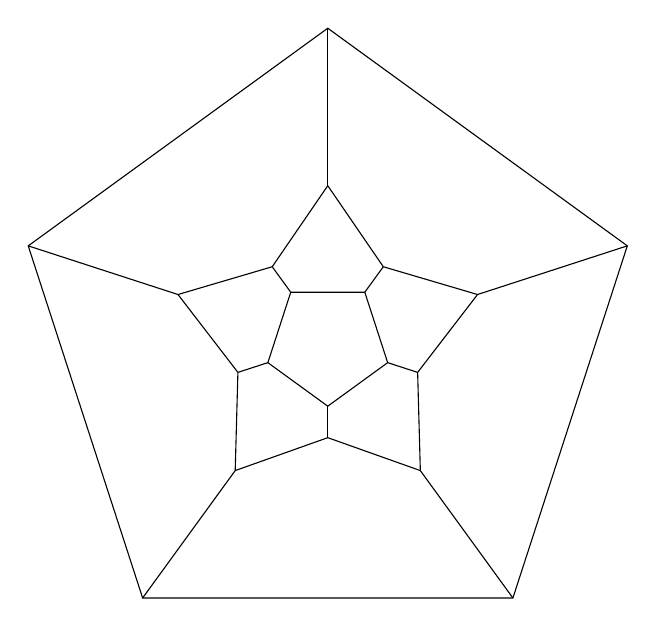
\begin{tikzpicture}
\coordinate (A) at ({(sqrt(10+2*sqrt(5)))},{(sqrt(5)-1)});
\coordinate (B) at (0,4);
\coordinate (C) at ({-(sqrt(10+2*sqrt(5)))},{(sqrt(5)-1)});
\coordinate (D) at ({-(sqrt(10-2*sqrt(5)))},{-(sqrt(5)+1)});
\coordinate (E) at ({(sqrt(10-2*sqrt(5)))},{-(sqrt(5)+1)});

\coordinate (F) at ({0.5*(sqrt(10+2*sqrt(5)))},{0.5*(sqrt(5)-1)});
\coordinate (G) at (0,2);
\coordinate (H) at ({-0.5*(sqrt(10+2*sqrt(5)))},{0.5*(sqrt(5)-1)});
\coordinate (I) at ({-0.5*(sqrt(10-2*sqrt(5)))},{-0.5*(sqrt(5)+1)});
\coordinate (J) at ({(0.5*sqrt(10-2*sqrt(5)))},{-0.5*(sqrt(5)+1)});

\coordinate (K) at ({-0.3*(sqrt(10+2*sqrt(5)))},{-0.3*(sqrt(5)-1)});
\coordinate (L) at (0,-1.2);
\coordinate (M) at ({0.3*(sqrt(10+2*sqrt(5)))},{-0.3*(sqrt(5)-1)});
\coordinate (N) at ({0.3*(sqrt(10-2*sqrt(5)))},{0.3*(sqrt(5)+1)});
\coordinate (O) at ({-0.3*(sqrt(10-2*sqrt(5)))},{0.3*(sqrt(5)+1)});

\coordinate (P) at ({-0.2*(sqrt(10+2*sqrt(5)))},{-0.2*(sqrt(5)-1)});
\coordinate (Q) at (0,-0.8);
\coordinate (R) at ({0.2*(sqrt(10+2*sqrt(5)))},{-0.2*(sqrt(5)-1)});
\coordinate (S) at ({0.2*(sqrt(10-2*sqrt(5)))},{0.2*(sqrt(5)+1)});
\coordinate (T) at ({-0.2*(sqrt(10-2*sqrt(5)))},{0.2*(sqrt(5)+1)});


\draw (A) -- (B) -- (C) -- (D) -- (E) -- cycle;
\draw (A) -- (F);
\draw (B) -- (G);
\draw (C) -- (H);
\draw (D) -- (I);
\draw (E) -- (J);

\draw (J) -- (L);
\draw (J) -- (M);
\draw (F) -- (M);
\draw (F) -- (N);
\draw (G) -- (N);
\draw (G) -- (O);
\draw (H) -- (O);
\draw (H) -- (K);
\draw (I) -- (K);
\draw (I) -- (L);

\draw (P) -- (Q) -- (R) -- (S) -- (T) -- cycle;
\draw (P) -- (K);
\draw (Q) -- (L);
\draw (R) -- (M);
\draw (S) -- (N);
\draw (T) -- (O);

  \end{tikzpicture}
  \caption{Dodekaeder.}
\end{figure}

\begin{figure}
\centering

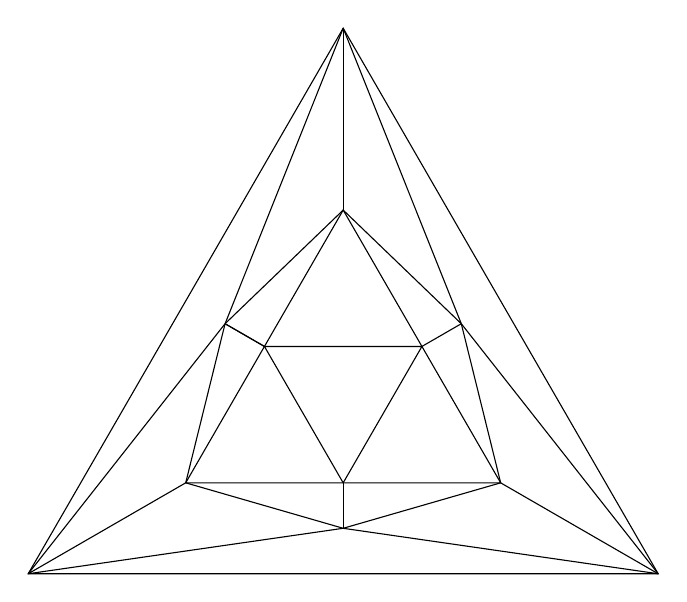
\begin{tikzpicture}[scale=2]
\coordinate (A) at (-2,0);
\coordinate (B) at (2,0);
\coordinate (C) at (0,{2*sqrt(3)});
\coordinate (D) at (-1,{sqrt(3)/3});
\coordinate (E) at (1,{sqrt(3)/3});
\coordinate (F) at (0,{4*sqrt(3)/3});
\coordinate (G) at (0,{sqrt(3)/3});
\coordinate (H) at (-0.5,{5*sqrt(3)/6});
\coordinate (I) at (0.5,{5*sqrt(3)/6});
\coordinate (J) at (0,{sqrt(3)/6});
\coordinate (K) at (-3/4,{11*sqrt(3)/12});
\coordinate (L) at (3/4,{11*sqrt(3)/12});

\draw (A) -- (B) -- (C) -- cycle;
\draw (A) -- (D);
\draw (B) -- (E);
\draw (C) -- (F);
\draw (D) -- (E) -- (F) -- cycle;
\draw (G) -- (H) -- (I) -- cycle;
\draw (A) -- (J);
\draw (A) -- (K);
\draw (B) -- (J);
\draw (B) -- (L);
\draw (C) -- (K);
\draw (C) -- (L);
\draw (K) -- (F);
\draw (K) -- (D);
\draw (J) -- (D);
\draw (J) -- (E);
\draw (L) -- (E);
\draw (L) -- (F);
\draw (L) -- (I);
\draw (K) -- (H);
\draw (K) -- (H);
\draw (J) -- (G);

\end{tikzpicture}
  \caption{Ikosaeder.}
  
\end{figure}
\end{losn}

\begin{oppg}
La $\{ p,q\}$ være Schläfli-symbolet til et regulært polyeder $P$. Vis at hvis $e$ er antall kanter, så er 
\[
\frac 1e = \frac 1p + \frac 1q - \frac 12.
\]
\end{oppg}
\begin{losn}
For det første: hver flate ligger på $p$ kanter, og det er $f$ flater. Men hver kant ligger på to flater, så $pf = 2e$. For det andre: hvert hjørne møter $q$ kanter, men hver kant har to hjørner, så $qv=2e$. I tillegg har vi Eulers formel som sier at $v-e+f=2$. Vi ønsker å eliminere $v$ og $f$, og få et uttrykk med bare $e,p,q$.

Vi har at $v = \frac{2e}{q}$ og at $f = \frac{2e}{p}$, så 
\[
\frac{2e}{q} - e + \frac{2e}{p} = 2.
\]
Gang uttrykket med $qp$ og få
\[
2ep - epq + 2eq = 2qp.
\]
Del på $2epq$:
\[
\frac{1}{q} - \frac{1}{2} + \frac{1}{p} = \frac{1}{e}.
\]
Som var det vi ønsket.
\end{losn}

\begin{oppg}
  La $P$ være et tredimensjonalt polyeder og la $\Gamma$ være kantgrafen til $P$. La $v_k$ være antall hjørner i $\Gamma$ med grad $k$. Anta $P$ har bare trekanter som sideflater og vis at 
\[
\sum_k \left( 1 - \frac k6 \right)v_k = 2.
\]
Generaliser, og vis at et polyeder med like kanter som sideflater bare kan ha enten trekanter, firkanter eller $5$-kanter som sideflater.
\end{oppg}
\begin{losn}
For det første ser vi at $\sum_k v_k = v$, siden vi ender opp med å summere over alle hjørnene. Dermed ser venstresiden av uttrykket ut som 
\[
v - \frac 16 \sum_k kv_k 
\]
Vi evaluerer summen ved å telle antall flater. Hvert hjørne av grad $k$ grenser til $k$ flater. Dermed finnes $kv_k$ flater med et hjørne av grad $k$ i ``midten'', hvor vi muligens har telt samme ting flere ganger. Summerer vi over alle $k$, har vi telt alle flatene, men vi har telt hver flate $3$ ganger siden flatene har tre hjørner. Så summen er lik $3f$. Dermed er uttrykket lik $v-\frac 12 f$. 

I tillegg: hver flate har $3$ kanter, så $3f$ teller alle flatene, men dobbelt opp (hver kant møter to flater), så $3f=2e$, og dermed er $-\frac 12 f = f - \frac 32  f = f - e$, slik at uttrykket vårt er lik $v+f-e$, som ved Eulers formel er lik $2$. Dermed har vi vist formelen.

Om nå $P$ hadde vært et polyeder med bare $n$-kanter, ser vi ved å gå gjennom argumentene over at formelen ville blitt:
\[
\sum_k \left( 1 - \frac{(n-2)k}{2n} \right)v_k = 2.
\]
Om polyederet bare hadde bestått av $n$-kanter med $n > 5$ skjer følgende: for det første: minst tre $n$-kanter må møtes i et hjørne, så første (potensielle) ikke-null ledd i summen er
\[
v_k \left( 1- \frac{(n-2)3}{2n} \right) = v_k \left( \frac{6-n}{2n} \right).
\]
Men denne summen er ikke positiv om $n \geq 6$. På samme måte ser vi at om $n \geq 6$, så vil venstresiden være negativ, og dermed kan den umulig bli positiv lik $2$. 
\end{losn}

\begin{oppg}
Finn $8$ punkter i $\R^3$ slik at den konvekse innhylningen av dem er en regulær kube. Bruk disse punktene til å finne koordinatene til hjørnene til et regulært tetraeder og et oktaeder.
\end{oppg}
\begin{losn}
En regulær kube er for eksempel lik innhylningen til de åtte punktene $(\pm 1,\pm 1, \pm 1)$. 

For å lage et tetraeder kan vi velge ett hjørne på kuben, for eksempel $(1,1,1)$. Langs diagonalene møter dette hjørnet tre andre hjørner. Eksplisitt er disse $(-1,1,1),(-1,-1,1)$ og $(-1,1,-1)$. (prøv og tegn!)

For å lage et oktaeder, velger vi midtpunktene på hver flate, og tar den konvekse innhylningen. Da får vi seks hjørner, gitt ved $(0,0,\pm 1)$, $(\pm 1,0,0)$ og $(0,\pm 1, 0)$.
\end{losn}

\end{document}
